% Input common header
\documentclass[xcolor=dvipsnames]{beamer}

\usecolortheme[named=Blue]{structure}
\setbeamertemplate{itemize items}[circle]

\usepackage{smartdiagram}


\author{Dr. Paul Larsen}
\date{\today}

\usetikzlibrary{decorations}
\usetikzlibrary{snakes}

\title{Artificial Intelligence, Risk and Discrete Geometry}
\begin{document}
\maketitle

\begin{frame}{Risk, Regulation and Artificial Intelligence\footnote{What about discrete geometry? Just wait \ldots it shows up soon and keeps reappearing}}
  \framesubtitle{\ldots in one diagram}
  \begin{center}
    \includegraphics[width=0.3\textheight]{graphics/exuberance-crisis-regulation}
  \end{center}
\end{frame}

\begin{frame}{What is Risk Regulation?}
  \framesubtitle{A brief history of financial disaster}
  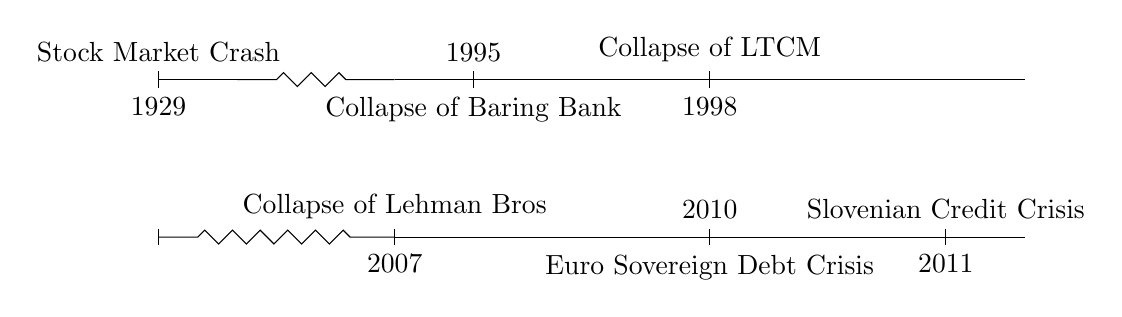
\begin{tikzpicture}[snake=zigzag, line before snake = 5mm, line after snake = 5mm]
    % draw horizontal line
    \draw (0,0) -- (1,0);
    \draw[snake] (1,0) -- (3,0);
    \draw (3,0) -- (11,0);
    % \draw[snake] (5,0) -- (7,0);

    % draw vertical lines
    \foreach \x in {0,4,7}
      \draw (\x cm,3pt) -- (\x cm,-3pt);

    % draw nodes
    \draw (0,0) node[below=3pt] {$ 1929 $} node[above=3pt] { Stock Market Crash };
    \draw (4,0) node[below=3pt] { Collapse of Baring Bank } node[above=3pt] {$ 1995 $};
    \draw (7,0) node[below=3pt] {$ 1998 $} node[above=3pt] { Collapse of LTCM };

    \draw[snake] (0,-2) -- (3,-2);
    \draw (3,-2) -- (11,-2);

    % draw vertical lines
    \foreach \x in {0,3,7,10}
      \draw (\x cm,-2.1) -- (\x cm,-1.9);

    % draw notes
    \draw (3,-2) node[below=3pt] {$ 2007 $} node[above=3pt] { Collapse of Lehman Bros };
    \draw (7,-2) node[below=3pt] { Euro Sovereign Debt Crisis } node[above=3pt] {$ 2010 $};
    \draw (10,-2) node[below=3pt] {$ 2011 $} node[above=3pt] { Slovenian Credit Crisis };
  %   \draw (6,0) node[below=3pt] {$  $} node[above=3pt] {$  $};
  %   \draw (7,0) node[below=3pt] {$ n $} node[above=3pt] {$ 10n $};
  \end{tikzpicture}
\end{frame}

\begin{frame}{What is Risk Regulation?}
  \framesubtitle{A cheeky guide to financial services risk types}
  \begin{block}{The risk of losing money due to \ldots}
    \begin{itemize}
      \item Credit: counter-party default
      \item Market: market movements
      \item Operational: something going wrong that shouldn't
      \item Liquidity: funding mismatches
      \item Insurance: unexpected loss of premiums or increase of claims
    \end{itemize}
  \end{block}

  \begin{block}{\ldots and the regulation that results from disasters big and small}
    \href{https://www.bis.org/basel_framework/}{Basil Framework (banking)},
    \href{https://www.eiopa.europa.eu/browse/solvency-2_en}{Solvency II (insurance)},
    \href{https://www.europarl.europa.eu/doceo/document/TA-9-2024-0138_EN.html}{The AI Act (EU)}
  \end{block}
\end{frame}


\begin{frame}{What is AI?}
\framesubtitle{Humans are amazing at navigating a world that does not make sense}
  \begin{tikzpicture}

    \node[inner sep=0pt] (grass) {
      \fbox{
          \includegraphics[width=0.7\textheight]{graphics/640px-Please_keep_off_the_grass_Great_Court_Trinity_College_Cambridge}
      }
    };
    \node[inner sep=0pt, right=0.5cm of grass] (door)  {
      \includegraphics[width=.4\textheight]{graphics/keep_door_closed}
    };

  \end{tikzpicture}

\end{frame}



%%%%%%%%%%%%
% AI Does Not Exist
%%%%%%%%%%%%
\begin{frame}[c]{What is AI?}
  \begin{center}
    \huge Artificial Intelligence Does Not Exist
  \end{center}

\vspace{0.5\textheight}
or so I claimed in the Spring, 2022 Workshop \ldots
\end{frame}

\begin{frame}{What is AI?}
  \framesubtitle{Artificial Intelligence does not exist, yet ...}
  \includegraphics[width=\textwidth]{graphics/tesla_paris}

  Source: \href{https://www.youtube.com/watch?v=_1MHGUC_BzQs}{YouTube: greentheonly, Paris streets in the eyes of Tesla Autopilot}
  \end{frame}

  \begin{frame}{What is AI?}
  \framesubtitle{Artificial Intelligence does not exist, yet ...}
  \includegraphics[width=\textwidth]{graphics/google_duplex}

  Source: \href{https://ai.googleblog.com/2018/05/duplex-ai-system-for-natural-conversation.html}{Google AI Blog}
\end{frame}

\begin{frame}{What is AI?}
  \framesubtitle{Artificial Intelligence does not exist, yet ...}
  \includegraphics[width=0.8\textwidth]{graphics/alpha_go}

  Source: \href{https://www.technologyreview.com/s/612923/how-alphazero-has-rewritten-the-rules-of-gameplay-on-its-own/}{MIT Technology Review}
\end{frame}

\begin{frame}{AI and Risk}
  \framesubtitle{AI struggles with context}
  \begin{columns}[T] % align columns
    \begin{column}{.45\textwidth}
      {\Large 2022 edition, GPT-2}:\newline

      The scientist named the population, after their distinctive horn, Ovid's Unicorn. These four-horned, silver-white unicorns were previously unknown to science.\newline

      Source: \href{https://www.lesswrong.com/posts/4AHXDwcGab5PhKhHT/humans-who-are-not-concentrating-are-not-general}{Humans Who Are Not Concentrating Are Not General Intelligences}

    \end{column}%
    \begin{column}{.45\textwidth}
      {\Large 2024 edition, GPT-4}:\newline
      \begin{center}
        \includegraphics[width=\textwidth]{graphics/melanie-mitchell-it-challenge}
      \end{center}

      Source of challenge: \cite{mitchell2019artificial}
    \end{column}%
\end{columns}

\end{frame}

\begin{frame}{AI and Risk}
  \framesubtitle{AI struggles with bias}
  \includegraphics[height=0.6\textheight]{graphics/facial_bias}

  Source: \href{https://www.nytimes.com/2018/02/09/technology/facial-recognition-race-artificial-intelligence.html}{New York Times}

  See also: \href{https://www.theverge.com/2018/1/12/16882408/google-racist-gorillas-photo-recognition-algorithm-ai}{James Vincent, The Verge, Google 'fixed' its racist algorithm by removing gorillas from its image-labeling tech}
\end{frame}

\begin{frame}{AI and Risk}
  \framesubtitle{AI Struggle\sout{s}d With Human Behavior (in 2022)}
  \begin{columns}[T] % align columns
    \begin{column}{.45\textwidth}
      {\Large 2022 edition, GPT-2}:\newline

      \href{run:graphics/siri_smart_sarcasm.m4a}{Siri Compliments}

      \begin{center}
        \includegraphics[height=0.6\textheight]{graphics/siri_transcript}
      \end{center}

    \end{column}%
    \begin{column}{.45\textwidth}
      {\Large 2024 edition, GPT-4}:\newline

      \href{run:graphics/chat-gpt-sarcasm.m4a}{ChatGPT Compliments}

      \begin{center}
        \includegraphics[height=0.6\textheight]{graphics/chat-gpt-4-sarcasm-transcript}
      \end{center}

    \end{column}%
\end{columns}
\end{frame}

\begin{frame}{AI: Where is the crisis?}
  \framesubtitle{High risk AI: education}
  \href{https://eur-lex.europa.eu/resource.html?uri=cellar:e0649735-a372-11eb-9585-01aa75ed71a1.0001.02/DOC_1&format=PDF}{Paragraph 35 of the AI Act} (emphasis added):
  \newline
  \begin{quotation}
    \noindent AI systems used in education or vocational training, notably for determining access or assigning persons to educational and vocational training institutions or to evaluate persons on tests as part of or as a precondition for their education should be considered high-risk.
  \end{quotation}
  \newline
  $\rightarrow$ \href{https://www.fastcompany.com/90342596/schools-are-quietly-turning-to-ai-to-help-pick-who-gets-in-what-could-go-wrong}{FastCompany: AI in admissions, what could go wrong?}
  \newline
  $\rightarrow$ \href{https://www.wired.com/story/algorithm-set-students-grades-altered-futures/}{Wired: The algorithms that keep students out of college}
  \newline
  $\rightarrow$ \href{https://www.theverge.com/2020/8/17/21372045/uk-a-level-results-algorithm-biased-coronavirus-covid-19-pandemic-university-applications}{Verge: UK ditches biased algorithm for university admission}

\end{frame}

\begin{frame}{AI: Where is the crisis?}
  \framesubtitle{High risk AI: access to finance}
  \href{https://eur-lex.europa.eu/resource.html?uri=cellar:e0649735-a372-11eb-9585-01aa75ed71a1.0001.02/DOC_1&format=PDF}{Paragraph 37 of the AI Act} (emphasis added):
  \begin{quotation}
    \noindent AI systems used to evaluate the credit score or creditworthiness of natural persons should be classified as high-risk AI systems, since they determine those persons \textcolor{red}{access to financial resources or essential services} such as housing, electricity, and telecommunication services. AI systems used for this purpose may lead to \textcolor{red}{discrimination} of persons or groups and \textcolor{red}{perpetuate historical patterns of discrimination}, for example based on racial or ethnic origins, disabilities, age, sexual orientation, or create new forms of discriminatory impacts.
  \end{quotation}
  \newline
  $\rightarrow$ \href{https://qz.com/1748321/the-role-of-goldman-sachs-algorithms-in-the-apple-credit-card-scandal/}{Apple Card Controversy: Is its algorithm biased against women?}
  \newline
  $\rightarrow$ \href{https://www.reubenbinns.com/blog/how-to-comply-with-gdpr-article-22-automated-credit-decisions/}{General Data Protection Regulation (EU) on automated credit decisions}
\end{frame}

\begin{frame}{AI: Where is the crisis?}
  \framesubtitle{\href{https://www.youtube.com/watch?v=5taE_br3Vr8}{Is AI "far more dangerous than nukes"?}}

From \href{https://futureoflife.org/open-letter/pause-giant-ai-experiments/}{Open Letter to AI Labs: Pause AI Experiments}\newline

\begin{quotation}
  \noindent [R]ecent months have seen AI labs locked in an out-of-control race to develop and deploy ever more powerful digital minds that no one – not even their creators – can understand, predict, or reliably control.

  \ldots

  \noindent Powerful AI systems should be developed only once we are confident that their effects will be positive and their risks will be manageable.
\end{quotation}

\end{frame}

\begin{frame}{AI: Where is the crisis?}
  \framesubtitle{\ldots and it is still about risk management}
  {\large Manage risk, don't eliminate it $\rightarrow$ risk and return}
  \newline
  \newline
  From the introduction of the \href{https://eur-lex.europa.eu/resource.html?uri=cellar:e0649735-a372-11eb-9585-01aa75ed71a1.0001.02/DOC_1&format=PDF}{AI Act} (emphasis added):
  \begin{quotation}
    \noindent By improving prediction, optimising operations and resource allocation, and personalising service delivery, the use of artificial intelligence can support \textcolor{red}{socially and environmentally beneficial outcomes} and provide key competitive advantages to companies and the European economy. Such action is especially needed in high-impact sectors, including climate change, environment and health, the public sector, finance, mobility, home affairs and agriculture. However, the same elements and techniques that power the socio-economic benefits of AI can also bring about \textcolor{red}{new risks or negative consequences for individuals or the society}.
  \end{quotation}

\end{frame}

\begin{frame}{AI: Where is the crisis?}
  \framesubtitle{\ldots and it is still about risk management, II}
  {\large Manage risk, don't eliminate it $\rightarrow$ risk and return}
  \newline
  \newline
  From mathematician \href{https://mathbabe.org/}{Cathy O'Neal}, author of \href{https://en.wikipedia.org/wiki/Weapons_of_Math_Destruction}{\textit{Weapons of Math Destruction}}, to \href{https://slate.com/business/2019/11/apple-card-credit-algorithm-bias-discrimination-women.html}{Slate} (emphasis added):
  \begin{quotation}
    \noindent \textcolor{red}{They look at the upside}—which is faster, scalable, quick decision-making—and \textcolor{red}{they ignore the downside}, which is that they're \textcolor{red}{taking on a lot of risk}.
  \end{quotation}

\end{frame}


\begin{frame}
\frametitle{Workshop topics}
\begin{enumerate}
\item Introduction
\item Discrete geometry for artificial intelligence and risk
\item Correlation and causation
\item Adversarial regularization regimes for classification tasks
\end{enumerate}
\end{frame}

\begin{frame}
\frametitle{Workshop format}

\begin{itemize}
\item For each topic, lecture + tutorial
\item Emphasis on examples with data produced via python package \href{https://munichpavel.github.io/fake-data-for-learning/}{fake-data-for-learning}
\item Light on non-mathematical definitions, thanks to
\end{itemize}
\centering
\includegraphics[width=0.3\textheight]{graphics/pi_wittgenstein}
\end{frame}

\begin{frame}[allowframebreaks]
  \frametitle{References}
  \setbeamertemplate{bibliography item}[text]
  \bibliographystyle{amsalpha}
  \bibliography{../references.bib}
\end{frame}



\end{document}